% Options for packages loaded elsewhere
\PassOptionsToPackage{unicode}{hyperref}
\PassOptionsToPackage{hyphens}{url}
\PassOptionsToPackage{dvipsnames,svgnames,x11names}{xcolor}
%
\documentclass[
  letterpaper,
  DIV=11,
  numbers=noendperiod]{scrartcl}

\usepackage{amsmath,amssymb}
\usepackage{lmodern}
\usepackage{iftex}
\ifPDFTeX
  \usepackage[T1]{fontenc}
  \usepackage[utf8]{inputenc}
  \usepackage{textcomp} % provide euro and other symbols
\else % if luatex or xetex
  \usepackage{unicode-math}
  \defaultfontfeatures{Scale=MatchLowercase}
  \defaultfontfeatures[\rmfamily]{Ligatures=TeX,Scale=1}
\fi
% Use upquote if available, for straight quotes in verbatim environments
\IfFileExists{upquote.sty}{\usepackage{upquote}}{}
\IfFileExists{microtype.sty}{% use microtype if available
  \usepackage[]{microtype}
  \UseMicrotypeSet[protrusion]{basicmath} % disable protrusion for tt fonts
}{}
\makeatletter
\@ifundefined{KOMAClassName}{% if non-KOMA class
  \IfFileExists{parskip.sty}{%
    \usepackage{parskip}
  }{% else
    \setlength{\parindent}{0pt}
    \setlength{\parskip}{6pt plus 2pt minus 1pt}}
}{% if KOMA class
  \KOMAoptions{parskip=half}}
\makeatother
\usepackage{xcolor}
\setlength{\emergencystretch}{3em} % prevent overfull lines
\setcounter{secnumdepth}{5}
% Make \paragraph and \subparagraph free-standing
\ifx\paragraph\undefined\else
  \let\oldparagraph\paragraph
  \renewcommand{\paragraph}[1]{\oldparagraph{#1}\mbox{}}
\fi
\ifx\subparagraph\undefined\else
  \let\oldsubparagraph\subparagraph
  \renewcommand{\subparagraph}[1]{\oldsubparagraph{#1}\mbox{}}
\fi

\usepackage{color}
\usepackage{fancyvrb}
\newcommand{\VerbBar}{|}
\newcommand{\VERB}{\Verb[commandchars=\\\{\}]}
\DefineVerbatimEnvironment{Highlighting}{Verbatim}{commandchars=\\\{\}}
% Add ',fontsize=\small' for more characters per line
\usepackage{framed}
\definecolor{shadecolor}{RGB}{241,243,245}
\newenvironment{Shaded}{\begin{snugshade}}{\end{snugshade}}
\newcommand{\AlertTok}[1]{\textcolor[rgb]{0.68,0.00,0.00}{#1}}
\newcommand{\AnnotationTok}[1]{\textcolor[rgb]{0.37,0.37,0.37}{#1}}
\newcommand{\AttributeTok}[1]{\textcolor[rgb]{0.40,0.45,0.13}{#1}}
\newcommand{\BaseNTok}[1]{\textcolor[rgb]{0.68,0.00,0.00}{#1}}
\newcommand{\BuiltInTok}[1]{\textcolor[rgb]{0.00,0.23,0.31}{#1}}
\newcommand{\CharTok}[1]{\textcolor[rgb]{0.13,0.47,0.30}{#1}}
\newcommand{\CommentTok}[1]{\textcolor[rgb]{0.37,0.37,0.37}{#1}}
\newcommand{\CommentVarTok}[1]{\textcolor[rgb]{0.37,0.37,0.37}{\textit{#1}}}
\newcommand{\ConstantTok}[1]{\textcolor[rgb]{0.56,0.35,0.01}{#1}}
\newcommand{\ControlFlowTok}[1]{\textcolor[rgb]{0.00,0.23,0.31}{#1}}
\newcommand{\DataTypeTok}[1]{\textcolor[rgb]{0.68,0.00,0.00}{#1}}
\newcommand{\DecValTok}[1]{\textcolor[rgb]{0.68,0.00,0.00}{#1}}
\newcommand{\DocumentationTok}[1]{\textcolor[rgb]{0.37,0.37,0.37}{\textit{#1}}}
\newcommand{\ErrorTok}[1]{\textcolor[rgb]{0.68,0.00,0.00}{#1}}
\newcommand{\ExtensionTok}[1]{\textcolor[rgb]{0.00,0.23,0.31}{#1}}
\newcommand{\FloatTok}[1]{\textcolor[rgb]{0.68,0.00,0.00}{#1}}
\newcommand{\FunctionTok}[1]{\textcolor[rgb]{0.28,0.35,0.67}{#1}}
\newcommand{\ImportTok}[1]{\textcolor[rgb]{0.00,0.46,0.62}{#1}}
\newcommand{\InformationTok}[1]{\textcolor[rgb]{0.37,0.37,0.37}{#1}}
\newcommand{\KeywordTok}[1]{\textcolor[rgb]{0.00,0.23,0.31}{#1}}
\newcommand{\NormalTok}[1]{\textcolor[rgb]{0.00,0.23,0.31}{#1}}
\newcommand{\OperatorTok}[1]{\textcolor[rgb]{0.37,0.37,0.37}{#1}}
\newcommand{\OtherTok}[1]{\textcolor[rgb]{0.00,0.23,0.31}{#1}}
\newcommand{\PreprocessorTok}[1]{\textcolor[rgb]{0.68,0.00,0.00}{#1}}
\newcommand{\RegionMarkerTok}[1]{\textcolor[rgb]{0.00,0.23,0.31}{#1}}
\newcommand{\SpecialCharTok}[1]{\textcolor[rgb]{0.37,0.37,0.37}{#1}}
\newcommand{\SpecialStringTok}[1]{\textcolor[rgb]{0.13,0.47,0.30}{#1}}
\newcommand{\StringTok}[1]{\textcolor[rgb]{0.13,0.47,0.30}{#1}}
\newcommand{\VariableTok}[1]{\textcolor[rgb]{0.07,0.07,0.07}{#1}}
\newcommand{\VerbatimStringTok}[1]{\textcolor[rgb]{0.13,0.47,0.30}{#1}}
\newcommand{\WarningTok}[1]{\textcolor[rgb]{0.37,0.37,0.37}{\textit{#1}}}

\providecommand{\tightlist}{%
  \setlength{\itemsep}{0pt}\setlength{\parskip}{0pt}}\usepackage{longtable,booktabs,array}
\usepackage{calc} % for calculating minipage widths
% Correct order of tables after \paragraph or \subparagraph
\usepackage{etoolbox}
\makeatletter
\patchcmd\longtable{\par}{\if@noskipsec\mbox{}\fi\par}{}{}
\makeatother
% Allow footnotes in longtable head/foot
\IfFileExists{footnotehyper.sty}{\usepackage{footnotehyper}}{\usepackage{footnote}}
\makesavenoteenv{longtable}
\usepackage{graphicx}
\makeatletter
\def\maxwidth{\ifdim\Gin@nat@width>\linewidth\linewidth\else\Gin@nat@width\fi}
\def\maxheight{\ifdim\Gin@nat@height>\textheight\textheight\else\Gin@nat@height\fi}
\makeatother
% Scale images if necessary, so that they will not overflow the page
% margins by default, and it is still possible to overwrite the defaults
% using explicit options in \includegraphics[width, height, ...]{}
\setkeys{Gin}{width=\maxwidth,height=\maxheight,keepaspectratio}
% Set default figure placement to htbp
\makeatletter
\def\fps@figure{htbp}
\makeatother
\newlength{\cslhangindent}
\setlength{\cslhangindent}{1.5em}
\newlength{\csllabelwidth}
\setlength{\csllabelwidth}{3em}
\newlength{\cslentryspacingunit} % times entry-spacing
\setlength{\cslentryspacingunit}{\parskip}
\newenvironment{CSLReferences}[2] % #1 hanging-ident, #2 entry spacing
 {% don't indent paragraphs
  \setlength{\parindent}{0pt}
  % turn on hanging indent if param 1 is 1
  \ifodd #1
  \let\oldpar\par
  \def\par{\hangindent=\cslhangindent\oldpar}
  \fi
  % set entry spacing
  \setlength{\parskip}{#2\cslentryspacingunit}
 }%
 {}
\usepackage{calc}
\newcommand{\CSLBlock}[1]{#1\hfill\break}
\newcommand{\CSLLeftMargin}[1]{\parbox[t]{\csllabelwidth}{#1}}
\newcommand{\CSLRightInline}[1]{\parbox[t]{\linewidth - \csllabelwidth}{#1}\break}
\newcommand{\CSLIndent}[1]{\hspace{\cslhangindent}#1}

\usepackage{booktabs}
\usepackage{longtable}
\usepackage{array}
\usepackage{multirow}
\usepackage{wrapfig}
\usepackage{float}
\usepackage{colortbl}
\usepackage{pdflscape}
\usepackage{tabu}
\usepackage{threeparttable}
\usepackage{threeparttablex}
\usepackage[normalem]{ulem}
\usepackage{makecell}
\usepackage{xcolor}
\KOMAoption{captions}{tableheading}
\makeatletter
\makeatother
\makeatletter
\makeatother
\makeatletter
\@ifpackageloaded{caption}{}{\usepackage{caption}}
\AtBeginDocument{%
\ifdefined\contentsname
  \renewcommand*\contentsname{Table of contents}
\else
  \newcommand\contentsname{Table of contents}
\fi
\ifdefined\listfigurename
  \renewcommand*\listfigurename{List of Figures}
\else
  \newcommand\listfigurename{List of Figures}
\fi
\ifdefined\listtablename
  \renewcommand*\listtablename{List of Tables}
\else
  \newcommand\listtablename{List of Tables}
\fi
\ifdefined\figurename
  \renewcommand*\figurename{Figure}
\else
  \newcommand\figurename{Figure}
\fi
\ifdefined\tablename
  \renewcommand*\tablename{Table}
\else
  \newcommand\tablename{Table}
\fi
}
\@ifpackageloaded{float}{}{\usepackage{float}}
\floatstyle{ruled}
\@ifundefined{c@chapter}{\newfloat{codelisting}{h}{lop}}{\newfloat{codelisting}{h}{lop}[chapter]}
\floatname{codelisting}{Listing}
\newcommand*\listoflistings{\listof{codelisting}{List of Listings}}
\makeatother
\makeatletter
\@ifpackageloaded{caption}{}{\usepackage{caption}}
\@ifpackageloaded{subcaption}{}{\usepackage{subcaption}}
\makeatother
\makeatletter
\@ifpackageloaded{tcolorbox}{}{\usepackage[many]{tcolorbox}}
\makeatother
\makeatletter
\@ifundefined{shadecolor}{\definecolor{shadecolor}{rgb}{.97, .97, .97}}
\makeatother
\makeatletter
\makeatother
\ifLuaTeX
  \usepackage{selnolig}  % disable illegal ligatures
\fi
\IfFileExists{bookmark.sty}{\usepackage{bookmark}}{\usepackage{hyperref}}
\IfFileExists{xurl.sty}{\usepackage{xurl}}{} % add URL line breaks if available
\urlstyle{same} % disable monospaced font for URLs
\hypersetup{
  pdftitle={Two-way split-plot design},
  colorlinks=true,
  linkcolor={blue},
  filecolor={Maroon},
  citecolor={Blue},
  urlcolor={Blue},
  pdfcreator={LaTeX via pandoc}}

\title{Two-way split-plot design}
\author{true}
\date{12/18/22}

\begin{document}
\maketitle
\begin{abstract}
Two-way ANOVA \& pairwise comparison post hoc tests in a split-plot
design.
\end{abstract}
\ifdefined\Shaded\renewenvironment{Shaded}{\begin{tcolorbox}[borderline west={3pt}{0pt}{shadecolor}, enhanced, sharp corners, frame hidden, breakable, interior hidden, boxrule=0pt]}{\end{tcolorbox}}\fi

\renewcommand*\contentsname{Table of contents}
{
\hypersetup{linkcolor=}
\setcounter{tocdepth}{3}
\tableofcontents
}
\begin{Shaded}
\begin{Highlighting}[]
\CommentTok{\# (install \&) load packages}
\NormalTok{pacman}\SpecialCharTok{::}\FunctionTok{p\_load}\NormalTok{(}
\NormalTok{  conflicted,}
\NormalTok{  desplot,}
\NormalTok{  emmeans,}
\NormalTok{  ggtext,}
\NormalTok{  lme4,}
\NormalTok{  lmerTest,}
\NormalTok{  MetBrewer,}
\NormalTok{  multcomp,}
\NormalTok{  multcompView,}
\NormalTok{  tidyverse)}

\CommentTok{\# handle function conflicts}
\FunctionTok{conflict\_prefer}\NormalTok{(}\StringTok{"filter"}\NormalTok{, }\StringTok{"dplyr"}\NormalTok{) }
\FunctionTok{conflict\_prefer}\NormalTok{(}\StringTok{"select"}\NormalTok{, }\StringTok{"dplyr"}\NormalTok{)}
\FunctionTok{conflict\_prefer}\NormalTok{(}\StringTok{"lmer"}\NormalTok{, }\StringTok{"lmerTest"}\NormalTok{)}
\end{Highlighting}
\end{Shaded}

\hypertarget{data}{%
\section{Data}\label{data}}

This dataset was originally published in Gomez and Gomez (1984) from a
yield (kg/ha) trial with 4 genotypes (\texttt{G}) and 6 nitrogen levels
(\texttt{N}), leading to 24 treatment level combinations. The data set
here has 3 complete replicates (\texttt{rep}) and is laid out as a
randomized complete block design (RCBD).

\hypertarget{import}{%
\subsection{Import}\label{import}}

\begin{Shaded}
\begin{Highlighting}[]
\NormalTok{\# data is available online:}
\NormalTok{path \textless{}{-} "https://raw.githubusercontent.com/SchmidtPaul/dsfair\_quarto/master/data/Gomez\&Gomez1984.csv"}
\end{Highlighting}
\end{Shaded}

\begin{Shaded}
\begin{Highlighting}[]
\NormalTok{dat }\OtherTok{\textless{}{-}} \FunctionTok{read\_csv}\NormalTok{(path) }\CommentTok{\# use path from above}
\NormalTok{dat}
\end{Highlighting}
\end{Shaded}

\begin{Shaded}
\begin{Highlighting}[]
\NormalTok{\# A tibble: 72 x 7}
\NormalTok{   yield   row   col rep   mainplot G     N     }
\NormalTok{   \textless{}dbl\textgreater{} \textless{}dbl\textgreater{} \textless{}dbl\textgreater{} \textless{}chr\textgreater{} \textless{}chr\textgreater{}    \textless{}chr\textgreater{} \textless{}chr\textgreater{} }
\NormalTok{ 1  4520     4     1 rep1  mp01     Simba Goomba}
\NormalTok{ 2  5598     2     2 rep1  mp02     Simba Koopa }
\NormalTok{ 3  6192     1     3 rep1  mp03     Simba Toad  }
\NormalTok{ 4  8542     2     4 rep1  mp04     Simba Peach }
\NormalTok{ 5  5806     2     5 rep1  mp05     Simba Diddy }
\NormalTok{ 6  7470     1     6 rep1  mp06     Simba Yoshi }
\NormalTok{ 7  4034     2     1 rep1  mp01     Nala  Goomba}
\NormalTok{ 8  6682     4     2 rep1  mp02     Nala  Koopa }
\NormalTok{ 9  6869     3     3 rep1  mp03     Nala  Toad  }
\NormalTok{10  6318     4     4 rep1  mp04     Nala  Peach }
\NormalTok{\# ... with 62 more rows}
\end{Highlighting}
\end{Shaded}

\hypertarget{format}{%
\subsection{Format}\label{format}}

Before anything, the columns \texttt{rep}, \texttt{N} and \texttt{G}
should be encoded as factors, since R by default encoded them as
character.

\begin{Shaded}
\begin{Highlighting}[]
\NormalTok{dat }\OtherTok{\textless{}{-}}\NormalTok{ dat }\SpecialCharTok{\%\textgreater{}\%}
  \FunctionTok{mutate}\NormalTok{(}\FunctionTok{across}\NormalTok{(}\FunctionTok{c}\NormalTok{(rep}\SpecialCharTok{:}\NormalTok{N), }\SpecialCharTok{\textasciitilde{}} \FunctionTok{as.factor}\NormalTok{(.x)))}
\end{Highlighting}
\end{Shaded}

\hypertarget{explore}{%
\subsection{Explore}\label{explore}}

We make use of
\href{../../summaryarticles/usefulthings.qmd\#dlookr}{\texttt{dlookr::describe()}}
to conveniently obtain descriptive summary tables. Here, we get can
summarize per nitrogen level, per genotype and also per
nitrogen-genotype-combination.

\begin{Shaded}
\begin{Highlighting}[]
\NormalTok{dat }\SpecialCharTok{\%\textgreater{}\%} 
  \FunctionTok{group\_by}\NormalTok{(N) }\SpecialCharTok{\%\textgreater{}\%} 
\NormalTok{  dlookr}\SpecialCharTok{::}\FunctionTok{describe}\NormalTok{(yield) }\SpecialCharTok{\%\textgreater{}\%} 
  \FunctionTok{select}\NormalTok{(}\DecValTok{2}\SpecialCharTok{:}\NormalTok{sd) }\SpecialCharTok{\%\textgreater{}\%}
  \FunctionTok{arrange}\NormalTok{(}\FunctionTok{desc}\NormalTok{(mean))}
\end{Highlighting}
\end{Shaded}

\begin{Shaded}
\begin{Highlighting}[]
\NormalTok{\# A tibble: 6 x 5}
\NormalTok{  N          n    na  mean    sd}
\NormalTok{  \textless{}fct\textgreater{}  \textless{}int\textgreater{} \textless{}int\textgreater{} \textless{}dbl\textgreater{} \textless{}dbl\textgreater{}}
\NormalTok{1 Diddy     12     0 5866.  832.}
\NormalTok{2 Toad      12     0 5864. 1434.}
\NormalTok{3 Yoshi     12     0 5812  2349.}
\NormalTok{4 Peach     12     0 5797. 2660.}
\NormalTok{5 Koopa     12     0 5478.  657.}
\NormalTok{6 Goomba    12     0 4054.  672.}
\end{Highlighting}
\end{Shaded}

\begin{Shaded}
\begin{Highlighting}[]
\NormalTok{dat }\SpecialCharTok{\%\textgreater{}\%} 
  \FunctionTok{group\_by}\NormalTok{(G) }\SpecialCharTok{\%\textgreater{}\%} 
\NormalTok{  dlookr}\SpecialCharTok{::}\FunctionTok{describe}\NormalTok{(yield) }\SpecialCharTok{\%\textgreater{}\%} 
  \FunctionTok{select}\NormalTok{(}\DecValTok{2}\SpecialCharTok{:}\NormalTok{sd) }\SpecialCharTok{\%\textgreater{}\%}
  \FunctionTok{arrange}\NormalTok{(}\FunctionTok{desc}\NormalTok{(mean))}
\end{Highlighting}
\end{Shaded}

\begin{Shaded}
\begin{Highlighting}[]
\NormalTok{\# A tibble: 4 x 5}
\NormalTok{  G         n    na  mean    sd}
\NormalTok{  \textless{}fct\textgreater{} \textless{}int\textgreater{} \textless{}int\textgreater{} \textless{}dbl\textgreater{} \textless{}dbl\textgreater{}}
\NormalTok{1 Simba    18     0 6554. 1475.}
\NormalTok{2 Nala     18     0 6156. 1078.}
\NormalTok{3 Timon    18     0 5563. 1269.}
\NormalTok{4 Pumba    18     0 3642. 1434.}
\end{Highlighting}
\end{Shaded}

\begin{Shaded}
\begin{Highlighting}[]
\NormalTok{dat }\SpecialCharTok{\%\textgreater{}\%} 
  \FunctionTok{group\_by}\NormalTok{(N, G) }\SpecialCharTok{\%\textgreater{}\%} 
\NormalTok{  dlookr}\SpecialCharTok{::}\FunctionTok{describe}\NormalTok{(yield) }\SpecialCharTok{\%\textgreater{}\%} 
  \FunctionTok{select}\NormalTok{(}\DecValTok{2}\SpecialCharTok{:}\NormalTok{sd) }\SpecialCharTok{\%\textgreater{}\%}
  \FunctionTok{arrange}\NormalTok{(}\FunctionTok{desc}\NormalTok{(mean)) }\SpecialCharTok{\%\textgreater{}\%} 
  \FunctionTok{print}\NormalTok{(}\AttributeTok{n=}\ConstantTok{Inf}\NormalTok{)}
\end{Highlighting}
\end{Shaded}

\begin{Shaded}
\begin{Highlighting}[]
\NormalTok{\# A tibble: 24 x 6}
\NormalTok{   N      G         n    na  mean     sd}
\NormalTok{   \textless{}fct\textgreater{}  \textless{}fct\textgreater{} \textless{}int\textgreater{} \textless{}int\textgreater{} \textless{}dbl\textgreater{}  \textless{}dbl\textgreater{}}
\NormalTok{ 1 Peach  Simba     3     0 8701.  270. }
\NormalTok{ 2 Yoshi  Simba     3     0 7563.   86.9}
\NormalTok{ 3 Yoshi  Nala      3     0 6951.  808. }
\NormalTok{ 4 Toad   Nala      3     0 6895   166. }
\NormalTok{ 5 Toad   Simba     3     0 6733.  490. }
\NormalTok{ 6 Yoshi  Timon     3     0 6687.  496. }
\NormalTok{ 7 Peach  Nala      3     0 6540.  936. }
\NormalTok{ 8 Diddy  Simba     3     0 6400   523. }
\NormalTok{ 9 Diddy  Nala      3     0 6259   499. }
\NormalTok{10 Peach  Timon     3     0 6065. 1097. }
\NormalTok{11 Toad   Timon     3     0 6014   515. }
\NormalTok{12 Diddy  Timon     3     0 5994   101. }
\NormalTok{13 Koopa  Nala      3     0 5982   684. }
\NormalTok{14 Koopa  Simba     3     0 5672   458. }
\NormalTok{15 Koopa  Timon     3     0 5443.  589. }
\NormalTok{16 Koopa  Pumba     3     0 4816   506. }
\NormalTok{17 Diddy  Pumba     3     0 4812   963. }
\NormalTok{18 Goomba Pumba     3     0 4481.  463. }
\NormalTok{19 Goomba Nala      3     0 4306   646. }
\NormalTok{20 Goomba Simba     3     0 4253.  248. }
\NormalTok{21 Toad   Pumba     3     0 3816  1311. }
\NormalTok{22 Goomba Timon     3     0 3177.  453. }
\NormalTok{23 Yoshi  Pumba     3     0 2047.  703. }
\NormalTok{24 Peach  Pumba     3     0 1881.  407. }
\end{Highlighting}
\end{Shaded}

Additionally, we can decide to plot our data. One way to deal with the
combination of two factors would be to use
\href{https://ggplot2.tidyverse.org/reference/facet_grid.html}{panels/facets
in ggplot2}.

Note that we here define a custom set of colors for the Nitrogen levels
that will be used throughout this chapter.

\begin{Shaded}
\begin{Highlighting}[]
\NormalTok{Ncolors }\OtherTok{\textless{}{-}} \FunctionTok{met.brewer}\NormalTok{(}\StringTok{"VanGogh2"}\NormalTok{, }\DecValTok{6}\NormalTok{) }\SpecialCharTok{\%\textgreater{}\%} 
  \FunctionTok{as.vector}\NormalTok{() }\SpecialCharTok{\%\textgreater{}\%} 
  \FunctionTok{set\_names}\NormalTok{(}\FunctionTok{levels}\NormalTok{(dat}\SpecialCharTok{$}\NormalTok{N))}
\end{Highlighting}
\end{Shaded}

\begin{Shaded}
\begin{Highlighting}[]
\FunctionTok{ggplot}\NormalTok{(}\AttributeTok{data =}\NormalTok{ dat) }\SpecialCharTok{+}
  \FunctionTok{aes}\NormalTok{(}\AttributeTok{y =}\NormalTok{ yield, }\AttributeTok{x =}\NormalTok{ N, }\AttributeTok{color =}\NormalTok{ N) }\SpecialCharTok{+}
  \FunctionTok{facet\_wrap}\NormalTok{(}\SpecialCharTok{\textasciitilde{}}\NormalTok{G, }\AttributeTok{labeller =}\NormalTok{ label\_both) }\SpecialCharTok{+}
  \FunctionTok{stat\_summary}\NormalTok{(}
    \AttributeTok{fun =}\NormalTok{ mean,}
    \AttributeTok{colour =} \StringTok{"grey"}\NormalTok{,}
    \AttributeTok{geom =} \StringTok{"line"}\NormalTok{,}
    \AttributeTok{linetype =} \StringTok{"dotted"}\NormalTok{,}
    \AttributeTok{group =} \DecValTok{1}
\NormalTok{  ) }\SpecialCharTok{+}
  \FunctionTok{geom\_point}\NormalTok{() }\SpecialCharTok{+}
  \FunctionTok{scale\_x\_discrete}\NormalTok{(}
    \AttributeTok{name =} \StringTok{"Nitrogen"}
\NormalTok{  ) }\SpecialCharTok{+}
  \FunctionTok{scale\_y\_continuous}\NormalTok{(}
    \AttributeTok{name =} \StringTok{"Yield"}\NormalTok{,}
    \AttributeTok{limits =} \FunctionTok{c}\NormalTok{(}\DecValTok{0}\NormalTok{, }\ConstantTok{NA}\NormalTok{),}
    \AttributeTok{expand =} \FunctionTok{expansion}\NormalTok{(}\AttributeTok{mult =} \FunctionTok{c}\NormalTok{(}\DecValTok{0}\NormalTok{, }\FloatTok{0.1}\NormalTok{))}
\NormalTok{  ) }\SpecialCharTok{+}
  \FunctionTok{scale\_color\_manual}\NormalTok{(}
    \AttributeTok{values =}\NormalTok{ Ncolors, }
    \AttributeTok{guide =} \StringTok{"none"}
\NormalTok{  ) }\SpecialCharTok{+}
  \FunctionTok{theme\_bw}\NormalTok{() }\SpecialCharTok{+}
  \FunctionTok{theme}\NormalTok{(}\AttributeTok{axis.text.x =} \FunctionTok{element\_text}\NormalTok{(}
    \AttributeTok{angle =} \DecValTok{45}\NormalTok{,}
    \AttributeTok{hjust =} \DecValTok{1}\NormalTok{,}
    \AttributeTok{vjust =} \DecValTok{1}
\NormalTok{  ))}
\end{Highlighting}
\end{Shaded}

\begin{figure}[H]

{\centering 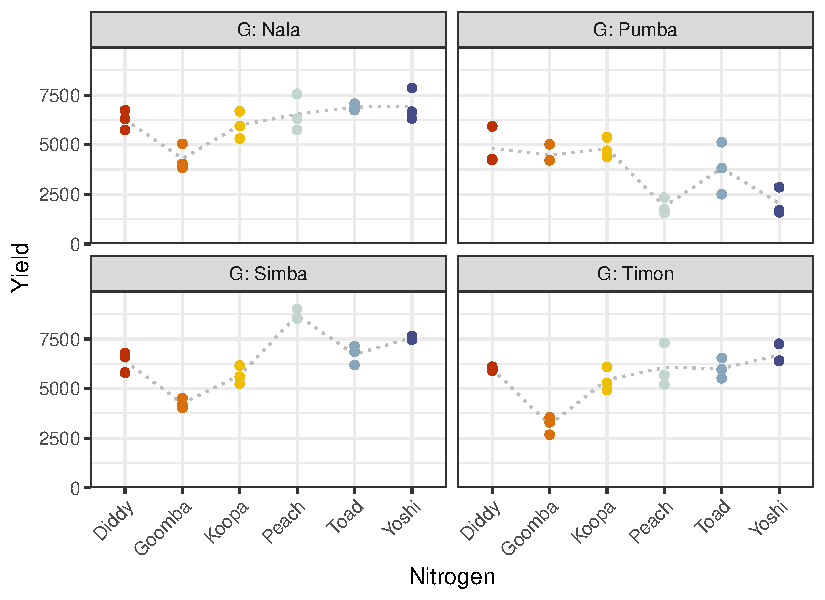
\includegraphics{splitplot_gomezgomez1984_files/figure-pdf/unnamed-chunk-9-1.pdf}

}

\end{figure}

Finally, since this is an experiment that was laid with a certain
experimental design (= a split-plot design) - it makes sense to also get
a field plan. This can be done via \texttt{desplot()} from
\href{../../summaryarticles/usefulthings.qmd\#desplot}{\{desplot\}}.

\begin{Shaded}
\begin{Highlighting}[]
\FunctionTok{desplot}\NormalTok{(}
  \AttributeTok{data =}\NormalTok{ dat,}
  \AttributeTok{form =}\NormalTok{ rep }\SpecialCharTok{\textasciitilde{}}\NormalTok{ col }\SpecialCharTok{+}\NormalTok{ row }\SpecialCharTok{|}\NormalTok{ rep, }\CommentTok{\# fill color per rep, headers per rep}
  \AttributeTok{col.regions =} \FunctionTok{c}\NormalTok{(}\StringTok{"white"}\NormalTok{, }\StringTok{"grey95"}\NormalTok{, }\StringTok{"grey90"}\NormalTok{),}
  \AttributeTok{text =}\NormalTok{ G, }\CommentTok{\# genotype names per plot}
  \AttributeTok{cex =} \FloatTok{0.8}\NormalTok{, }\CommentTok{\# genotype names: font size}
  \AttributeTok{shorten =} \StringTok{"abb"}\NormalTok{, }\CommentTok{\# genotype names: abbreviate}
  \AttributeTok{col =}\NormalTok{ N, }\CommentTok{\# color of genotype names for each N{-}level}
  \AttributeTok{col.text =}\NormalTok{ Ncolors, }\CommentTok{\# use custom colors from above}
  \AttributeTok{out1 =}\NormalTok{ col, }\AttributeTok{out1.gpar =} \FunctionTok{list}\NormalTok{(}\AttributeTok{col =} \StringTok{"darkgrey"}\NormalTok{), }\CommentTok{\# lines between columns}
  \AttributeTok{out2 =}\NormalTok{ row, }\AttributeTok{out2.gpar =} \FunctionTok{list}\NormalTok{(}\AttributeTok{col =} \StringTok{"darkgrey"}\NormalTok{), }\CommentTok{\# lines between rows}
  \AttributeTok{main =} \StringTok{"Field layout"}\NormalTok{, }\CommentTok{\# plot title}
  \AttributeTok{show.key =} \ConstantTok{TRUE}\NormalTok{, }\CommentTok{\# show legend}
  \AttributeTok{key.cex =} \FloatTok{0.7} \CommentTok{\# legend font size}
\NormalTok{  )}
\end{Highlighting}
\end{Shaded}

\begin{figure}[H]

{\centering 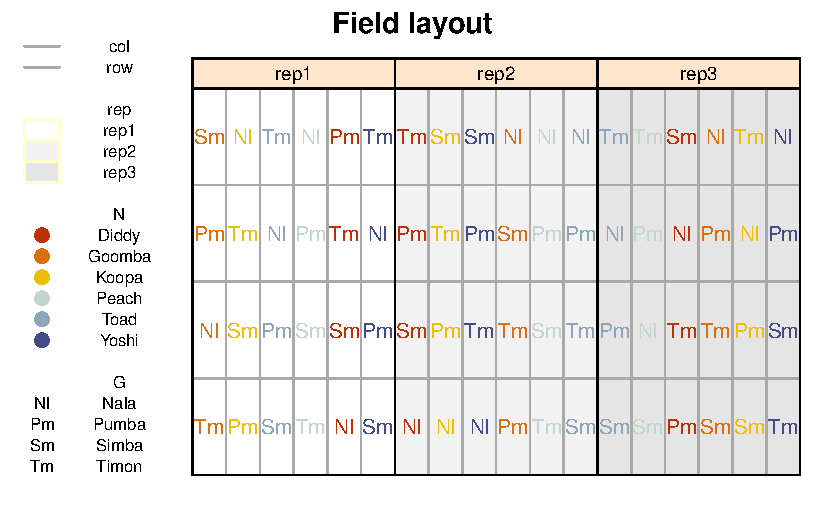
\includegraphics{splitplot_gomezgomez1984_files/figure-pdf/unnamed-chunk-10-1.pdf}

}

\end{figure}

\begin{Shaded}
\begin{Highlighting}[]
\FunctionTok{desplot}\NormalTok{(}
  \AttributeTok{data =}\NormalTok{ dat,}
  \AttributeTok{form =}\NormalTok{ yield }\SpecialCharTok{\textasciitilde{}}\NormalTok{ col }\SpecialCharTok{+}\NormalTok{ row }\SpecialCharTok{|}\NormalTok{ rep, }\CommentTok{\# fill color per rep, headers per rep}
  \AttributeTok{text =}\NormalTok{ G, }\CommentTok{\# genotype names per plot}
  \AttributeTok{cex =} \FloatTok{0.8}\NormalTok{, }\CommentTok{\# genotype names: font size}
  \AttributeTok{shorten =} \StringTok{"abb"}\NormalTok{, }\CommentTok{\# genotype names: abbreviate}
  \AttributeTok{col  =}\NormalTok{ N, }\CommentTok{\# color of genotype names for each N{-}level}
  \AttributeTok{col.text =}\NormalTok{ Ncolors, }\CommentTok{\# use custom colors from above}
  \AttributeTok{out1 =}\NormalTok{ col, }\AttributeTok{out1.gpar =} \FunctionTok{list}\NormalTok{(}\AttributeTok{col =} \StringTok{"darkgrey"}\NormalTok{), }\CommentTok{\# lines between columns}
  \AttributeTok{out2 =}\NormalTok{ row, }\AttributeTok{out2.gpar =} \FunctionTok{list}\NormalTok{(}\AttributeTok{col =} \StringTok{"darkgrey"}\NormalTok{), }\CommentTok{\# lines between rows}
  \AttributeTok{main =} \StringTok{"Yield per plot"}\NormalTok{, }\CommentTok{\# plot title}
  \AttributeTok{show.key =} \ConstantTok{FALSE} \CommentTok{\# show legend}
\NormalTok{  )}
\end{Highlighting}
\end{Shaded}

\begin{figure}[H]

{\centering 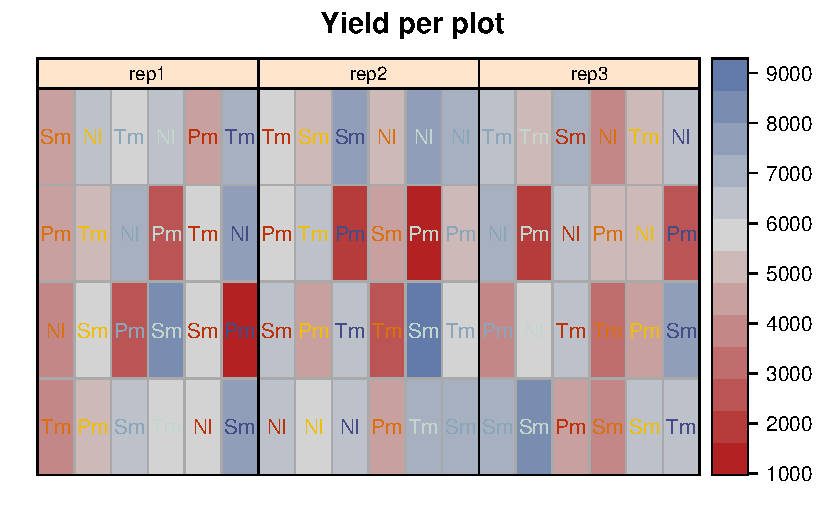
\includegraphics{splitplot_gomezgomez1984_files/figure-pdf/unnamed-chunk-11-1.pdf}

}

\end{figure}

\begin{Shaded}
\begin{Highlighting}[]
\NormalTok{mainplotcolors }\OtherTok{\textless{}{-}} \FunctionTok{c}\NormalTok{(}\FunctionTok{met.brewer}\NormalTok{(}\StringTok{"VanGogh3"}\NormalTok{, }\DecValTok{6}\NormalTok{),}
                    \FunctionTok{met.brewer}\NormalTok{(}\StringTok{"Hokusai2"}\NormalTok{, }\DecValTok{6}\NormalTok{),}
                    \FunctionTok{met.brewer}\NormalTok{(}\StringTok{"OKeeffe2"}\NormalTok{, }\DecValTok{6}\NormalTok{)) }\SpecialCharTok{\%\textgreater{}\%}
  \FunctionTok{as.vector}\NormalTok{() }\SpecialCharTok{\%\textgreater{}\%}
  \FunctionTok{set\_names}\NormalTok{(}\FunctionTok{levels}\NormalTok{(dat}\SpecialCharTok{$}\NormalTok{mainplot))}

\FunctionTok{desplot}\NormalTok{(}
  \AttributeTok{data =}\NormalTok{ dat,}
  \AttributeTok{form =}\NormalTok{ mainplot }\SpecialCharTok{\textasciitilde{}}\NormalTok{ col }\SpecialCharTok{+}\NormalTok{ row }\SpecialCharTok{|}\NormalTok{ rep, }\CommentTok{\# fill color per rep, headers per rep}
  \AttributeTok{col.regions =}\NormalTok{ mainplotcolors,}
  \AttributeTok{out1 =}\NormalTok{ col, }\AttributeTok{out1.gpar =} \FunctionTok{list}\NormalTok{(}\AttributeTok{col =} \StringTok{"darkgrey"}\NormalTok{), }\CommentTok{\# lines between columns}
  \AttributeTok{out2 =}\NormalTok{ row, }\AttributeTok{out2.gpar =} \FunctionTok{list}\NormalTok{(}\AttributeTok{col =} \StringTok{"darkgrey"}\NormalTok{), }\CommentTok{\# lines between rows}
  \AttributeTok{main =} \StringTok{"Experimental design focus"}\NormalTok{, }\CommentTok{\# plot title}
  \AttributeTok{show.key =} \ConstantTok{TRUE}\NormalTok{, }\CommentTok{\# don\textquotesingle{}t show legend}
  \AttributeTok{key.cex =} \FloatTok{0.5}
\NormalTok{  )}
\end{Highlighting}
\end{Shaded}

\begin{figure}[H]

{\centering 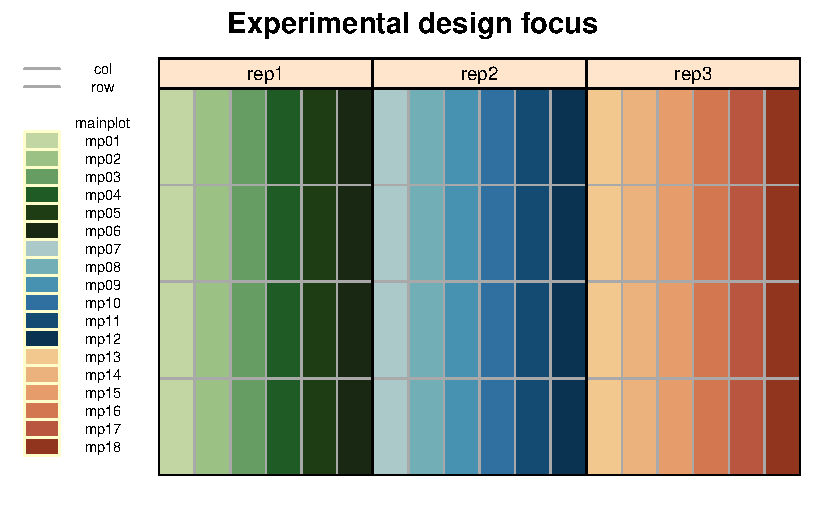
\includegraphics{splitplot_gomezgomez1984_files/figure-pdf/unnamed-chunk-12-1.pdf}

}

\end{figure}

\hypertarget{model}{%
\section{Model}\label{model}}

Finally, we can decide to fit a linear model with yield as the response
variable. In this example it makes sense to mentally group the effects
in our model as either \emph{design effects} or \emph{treatment
effects}. The treatments here are the genotypes \texttt{G} and the
nitrogen levels \texttt{N} which we will include in the model as main
effects, but also via their interaction effect \texttt{N:G}. Regarding
the design, the model needs to contain a block (\texttt{rep}) effect
representing the three complete blocks. Additionally, there should also
be random effects for the 18 mainplots, since they represent additional
randomization units.

\begin{Shaded}
\begin{Highlighting}[]
\NormalTok{mod }\OtherTok{\textless{}{-}} \FunctionTok{lmer}\NormalTok{(yield }\SpecialCharTok{\textasciitilde{}}\NormalTok{ G }\SpecialCharTok{+}\NormalTok{ N }\SpecialCharTok{+}\NormalTok{ G}\SpecialCharTok{:}\NormalTok{N }\SpecialCharTok{+}
\NormalTok{              rep }\SpecialCharTok{+}\NormalTok{ (}\DecValTok{1} \SpecialCharTok{|}\NormalTok{ rep}\SpecialCharTok{:}\NormalTok{mainplot),}
            \AttributeTok{data =}\NormalTok{ dat)}
\end{Highlighting}
\end{Shaded}

It would be at this moment (i.e.~after fitting the model and before
running the ANOVA), that you should check whether the model assumptions
are met. Find out more in the
\href{../../summaryarticles/modeldiagnostics.qmd}{summary article
``Model Diagnostics''}

\hypertarget{anova}{%
\section{ANOVA}\label{anova}}

Based on our model, we can then conduct an ANOVA:

\begin{Shaded}
\begin{Highlighting}[]
\NormalTok{ANOVA }\OtherTok{\textless{}{-}} \FunctionTok{anova}\NormalTok{(mod)}
\NormalTok{ANOVA}
\end{Highlighting}
\end{Shaded}

\begin{Shaded}
\begin{Highlighting}[]
\NormalTok{Type III Analysis of Variance Table with Satterthwaite\textquotesingle{}s method}
\NormalTok{      Sum Sq  Mean Sq NumDF DenDF F value    Pr(\textgreater{}F)    }
\NormalTok{G   89885051 29961684     3    36 85.7416 \textless{} 2.2e{-}16 ***}
\NormalTok{N   19192886  3838577     5    10 10.9849 0.0008277 ***}
\NormalTok{rep   683088   341544     2    10  0.9774 0.4095330    }
\NormalTok{G:N 69378044  4625203    15    36 13.2360 2.078e{-}10 ***}
\NormalTok{{-}{-}{-}}
\NormalTok{Signif. codes:  0 \textquotesingle{}***\textquotesingle{} 0.001 \textquotesingle{}**\textquotesingle{} 0.01 \textquotesingle{}*\textquotesingle{} 0.05 \textquotesingle{}.\textquotesingle{} 0.1 \textquotesingle{} \textquotesingle{} 1}
\end{Highlighting}
\end{Shaded}

Accordingly, the ANOVA's F-test found the nitrogen-genotype-interaction
to be statistically different (p \textless{} .001***).

\hypertarget{mean-comparison}{%
\section{Mean comparison}\label{mean-comparison}}

Besides an ANOVA, one may also want to compare adjusted yield means
between cultivars via post hoc tests (t-test, Tukey test etc.).
Especially because of the results of this ANOVA, we should compare means
for all \texttt{N:G} interactions and \textbf{not} for the \texttt{N}
and/or \texttt{G} main effects. When doing so, we still have multiple
options to choose from. I here decide to compare all genotype means per
nitrogen

\begin{Shaded}
\begin{Highlighting}[]
\NormalTok{mean\_comp }\OtherTok{\textless{}{-}}\NormalTok{ mod }\SpecialCharTok{\%\textgreater{}\%} 
  \FunctionTok{emmeans}\NormalTok{(}\AttributeTok{specs =} \SpecialCharTok{\textasciitilde{}}\NormalTok{ N}\SpecialCharTok{|}\NormalTok{G) }\SpecialCharTok{\%\textgreater{}\%} \CommentTok{\# adj. mean per cultivar}
  \FunctionTok{cld}\NormalTok{(}\AttributeTok{Letters =}\NormalTok{ letters) }\CommentTok{\# compact letter display (CLD)}

\NormalTok{mean\_comp}
\end{Highlighting}
\end{Shaded}

\begin{Shaded}
\begin{Highlighting}[]
\NormalTok{G = Nala:}
\NormalTok{ N      emmean  SE   df lower.CL upper.CL .group}
\NormalTok{ Goomba   4306 366 41.9     3568     5044  a    }
\NormalTok{ Koopa    5982 366 41.9     5244     6720   b   }
\NormalTok{ Diddy    6259 366 41.9     5521     6997   b   }
\NormalTok{ Peach    6540 366 41.9     5803     7278   b   }
\NormalTok{ Toad     6895 366 41.9     6157     7633   b   }
\NormalTok{ Yoshi    6951 366 41.9     6213     7688   b   }

\NormalTok{G = Pumba:}
\NormalTok{ N      emmean  SE   df lower.CL upper.CL .group}
\NormalTok{ Peach    1881 366 41.9     1143     2618  a    }
\NormalTok{ Yoshi    2047 366 41.9     1309     2784  a    }
\NormalTok{ Toad     3816 366 41.9     3078     4554   b   }
\NormalTok{ Goomba   4481 366 41.9     3744     5219   b   }
\NormalTok{ Diddy    4812 366 41.9     4074     5550   b   }
\NormalTok{ Koopa    4816 366 41.9     4078     5554   b   }

\NormalTok{G = Simba:}
\NormalTok{ N      emmean  SE   df lower.CL upper.CL .group}
\NormalTok{ Goomba   4253 366 41.9     3515     4990  a    }
\NormalTok{ Koopa    5672 366 41.9     4934     6410  ab   }
\NormalTok{ Diddy    6400 366 41.9     5662     7138   bc  }
\NormalTok{ Toad     6733 366 41.9     5995     7470   bc  }
\NormalTok{ Yoshi    7563 366 41.9     6826     8301    cd }
\NormalTok{ Peach    8701 366 41.9     7963     9438     d }

\NormalTok{G = Timon:}
\NormalTok{ N      emmean  SE   df lower.CL upper.CL .group}
\NormalTok{ Goomba   3177 366 41.9     2440     3915  a    }
\NormalTok{ Koopa    5443 366 41.9     4705     6180   b   }
\NormalTok{ Diddy    5994 366 41.9     5256     6732   b   }
\NormalTok{ Toad     6014 366 41.9     5276     6752   b   }
\NormalTok{ Peach    6065 366 41.9     5328     6803   b   }
\NormalTok{ Yoshi    6687 366 41.9     5950     7425   b   }

\NormalTok{Results are averaged over the levels of: rep }
\NormalTok{Degrees{-}of{-}freedom method: kenward{-}roger }
\NormalTok{Confidence level used: 0.95 }
\NormalTok{P value adjustment: tukey method for comparing a family of 6 estimates }
\NormalTok{significance level used: alpha = 0.05 }
\NormalTok{NOTE: If two or more means share the same grouping symbol,}
\NormalTok{      then we cannot show them to be different.}
\NormalTok{      But we also did not show them to be the same. }
\end{Highlighting}
\end{Shaded}

Note that if you would like to see the underlying individual
contrasts/differences between adjusted means, simply add
\texttt{details\ =\ TRUE} to the \texttt{cld()} statement. Furthermore,
check out the
\href{../../summaryarticles/compactletterdisplay.qmd}{Summary Article
``Compact Letter Display''}.

Finally, we can create a plot that displays both the raw data and the
results, \emph{i.e.} the comparisons of the adjusted means that are
based on the linear model.

\begin{Shaded}
\begin{Highlighting}[]
\NormalTok{my\_caption }\OtherTok{\textless{}{-}} \StringTok{"The four facettes represent genotypes A, B, C and D. Black dots represent raw data. Red dots and error bars represent adjusted means with 95\% confidence limits per cultivar. For each genotype separately, means followed by a common letter are not significantly different according to the Tukey{-}test."}

\FunctionTok{ggplot}\NormalTok{() }\SpecialCharTok{+}
  \FunctionTok{facet\_wrap}\NormalTok{(}\SpecialCharTok{\textasciitilde{}}\NormalTok{G, }\AttributeTok{labeller =}\NormalTok{ label\_both) }\SpecialCharTok{+} \CommentTok{\# facette per G level}
  \FunctionTok{aes}\NormalTok{(}\AttributeTok{x =}\NormalTok{ N) }\SpecialCharTok{+}
  \CommentTok{\# black dots representing the raw data}
  \FunctionTok{geom\_point}\NormalTok{(}
    \AttributeTok{data =}\NormalTok{ dat,}
    \FunctionTok{aes}\NormalTok{(}\AttributeTok{y =}\NormalTok{ yield, }\AttributeTok{color =}\NormalTok{ N)}
\NormalTok{  ) }\SpecialCharTok{+}
  \CommentTok{\# red dots representing the adjusted means}
  \FunctionTok{geom\_point}\NormalTok{(}
    \AttributeTok{data =}\NormalTok{ mean\_comp,}
    \FunctionTok{aes}\NormalTok{(}\AttributeTok{y =}\NormalTok{ emmean),}
    \AttributeTok{color =} \StringTok{"red"}\NormalTok{,}
    \AttributeTok{position =} \FunctionTok{position\_nudge}\NormalTok{(}\AttributeTok{x =} \FloatTok{0.2}\NormalTok{)}
\NormalTok{  ) }\SpecialCharTok{+}
  \CommentTok{\# red error bars representing the confidence limits of the adjusted means}
  \FunctionTok{geom\_errorbar}\NormalTok{(}
    \AttributeTok{data =}\NormalTok{ mean\_comp,}
    \FunctionTok{aes}\NormalTok{(}\AttributeTok{ymin =}\NormalTok{ lower.CL, }\AttributeTok{ymax =}\NormalTok{ upper.CL),}
    \AttributeTok{color =} \StringTok{"red"}\NormalTok{,}
    \AttributeTok{width =} \FloatTok{0.1}\NormalTok{,}
    \AttributeTok{position =} \FunctionTok{position\_nudge}\NormalTok{(}\AttributeTok{x =} \FloatTok{0.2}\NormalTok{)}
\NormalTok{  ) }\SpecialCharTok{+}
  \CommentTok{\# red letters }
  \FunctionTok{geom\_text}\NormalTok{(}
    \AttributeTok{data =}\NormalTok{ mean\_comp,}
    \FunctionTok{aes}\NormalTok{(}\AttributeTok{y =}\NormalTok{ emmean, }\AttributeTok{label =} \FunctionTok{str\_trim}\NormalTok{(.group)),}
    \AttributeTok{color =} \StringTok{"red"}\NormalTok{,}
    \AttributeTok{position =} \FunctionTok{position\_nudge}\NormalTok{(}\AttributeTok{x =} \FloatTok{0.35}\NormalTok{),}
    \AttributeTok{hjust =} \DecValTok{0}
\NormalTok{  ) }\SpecialCharTok{+}
  \FunctionTok{scale\_x\_discrete}\NormalTok{(}
    \AttributeTok{name =} \StringTok{"Nitrogen"}
\NormalTok{  ) }\SpecialCharTok{+}
  \FunctionTok{scale\_y\_continuous}\NormalTok{(}
    \AttributeTok{name =} \StringTok{"Yield"}\NormalTok{,}
    \AttributeTok{limits =} \FunctionTok{c}\NormalTok{(}\DecValTok{0}\NormalTok{, }\ConstantTok{NA}\NormalTok{),}
    \AttributeTok{expand =} \FunctionTok{expansion}\NormalTok{(}\AttributeTok{mult =} \FunctionTok{c}\NormalTok{(}\DecValTok{0}\NormalTok{, }\FloatTok{0.1}\NormalTok{))}
\NormalTok{  ) }\SpecialCharTok{+}
  \FunctionTok{scale\_color\_manual}\NormalTok{(}
    \AttributeTok{values =}\NormalTok{ Ncolors, }
    \AttributeTok{guide =} \StringTok{"none"}
\NormalTok{  ) }\SpecialCharTok{+}
  \FunctionTok{theme\_bw}\NormalTok{() }\SpecialCharTok{+}
  \FunctionTok{labs}\NormalTok{(}\AttributeTok{caption =}\NormalTok{ my\_caption) }\SpecialCharTok{+}
  \FunctionTok{theme}\NormalTok{(}
    \AttributeTok{plot.caption =} \FunctionTok{element\_textbox\_simple}\NormalTok{(}\AttributeTok{margin =} \FunctionTok{margin}\NormalTok{(}\AttributeTok{t =} \DecValTok{5}\NormalTok{)),}
    \AttributeTok{plot.caption.position =} \StringTok{"plot"}\NormalTok{,}
    \AttributeTok{axis.text.x =} \FunctionTok{element\_text}\NormalTok{(}
      \AttributeTok{angle =} \DecValTok{45}\NormalTok{,}
      \AttributeTok{hjust =} \DecValTok{1}\NormalTok{,}
      \AttributeTok{vjust =} \DecValTok{1}
\NormalTok{    )}
\NormalTok{  )}
\end{Highlighting}
\end{Shaded}

\begin{figure}[H]

{\centering 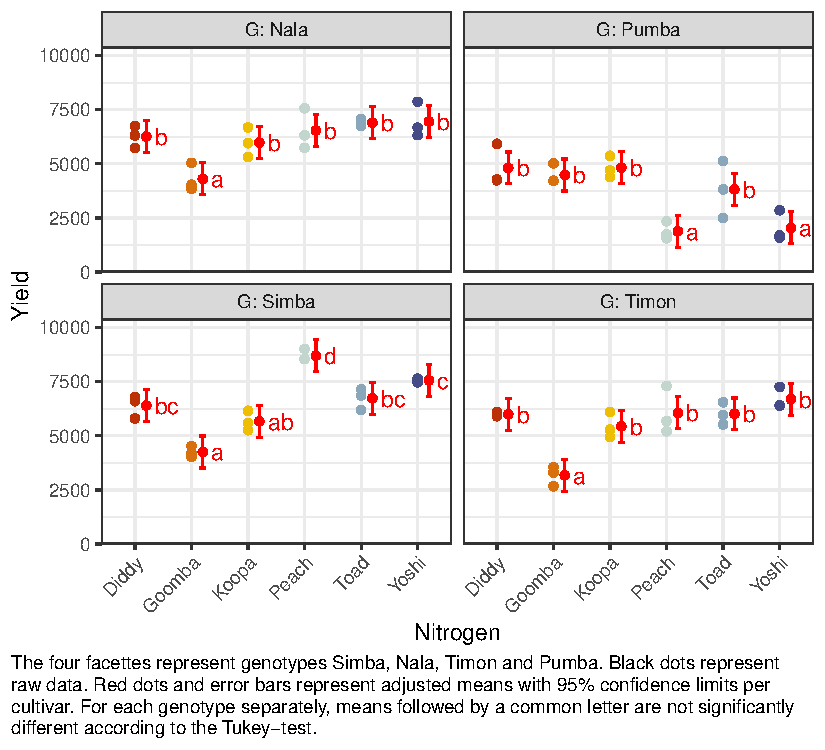
\includegraphics{splitplot_gomezgomez1984_files/figure-pdf/unnamed-chunk-16-1.pdf}

}

\end{figure}

\hypertarget{refs}{}
\begin{CSLReferences}{1}{0}
\leavevmode\vadjust pre{\hypertarget{ref-gomez1984}{}}%
Gomez, Kwanchai A, and Arturo A Gomez. 1984. \emph{Statistical
Procedures for Agricultural Research}. 2nd ed. An International Rice
Research Institute Book. Nashville, TN: John Wiley \& Sons.

\end{CSLReferences}



\end{document}
